Recall the general DAE representation:
\begin{equation}
E*dx = A*x + B*u + F*w + g
\end{equation}Introducing the ODE representation that also can be extracted:
\begin{equation}
dx = A*x + B*u + g
\end{equation}
\begin{equation}
w  = H*x + M*u + q
\end{equation}\newline Here it might be tempting to create the SFGs from the ODE instead, since one can extract the SFGs  for the states and algebraic variables separately. But notice, now the states does not depend at all on the algebraic variables in w. This is still a correct system, since algebraic variables is only a combination of states,other algebraic variables and constants thus can be reduced and replaced by other states and a constant. But even though it is mathematically correc, we have lost information. The causality is broken, and a user that has declared states that depends on algebraic variables can no longer view and analyse such relations inside ProMoVis. If we consider the following, fictional, system:

\begin{equation}
dx_1=x2+w_1+u_2
\end{equation}
\begin{equation}
dx_2=x3+u_1
\end{equation}
\begin{equation}
dx_3=x1
\end{equation}
\begin{equation}
w_1=x3+x2
\end{equation}\newline The DAE representation of this system is then:\\\newline
$
\begin{bmatrix}  1 & 0 & 0 \\ 0 & 1 & 0  \\ 0 & 0 & 1 \\ 0 & 0 & 0   \end{bmatrix} \times \left[ \begin{array}{c} dx_1 \\ dx_2 \\ dx_3 \end{array} \right]
= \begin{bmatrix} 0 & 1 & 0 \\ 0 & 0 & 1 \\ 1 & 0 & 0 \\ 0 & 1 & 1 \end{bmatrix} \times \left[ \begin{array}{c} x_1 \\ x_2 \\ x_3 \end{array} \right] + \begin{bmatrix} 0 & 1 \\ 1 & 0 \\ 0 & 0 \\ 0 & 0 \end{bmatrix} \times \left[ \begin{array}{c} u_1 \\ u_2 \end{array} \right]+
\begin{bmatrix} 1 \\ 0 \\ 0  \\ -1 \end{bmatrix} \times \left[ \begin{array}{c} w_1 \end{array} \right]$\newline
And has the corresponding SFG:\newline
\setlength\fboxsep{0pt}
\setlength\fboxrule{0.5pt}
\fbox{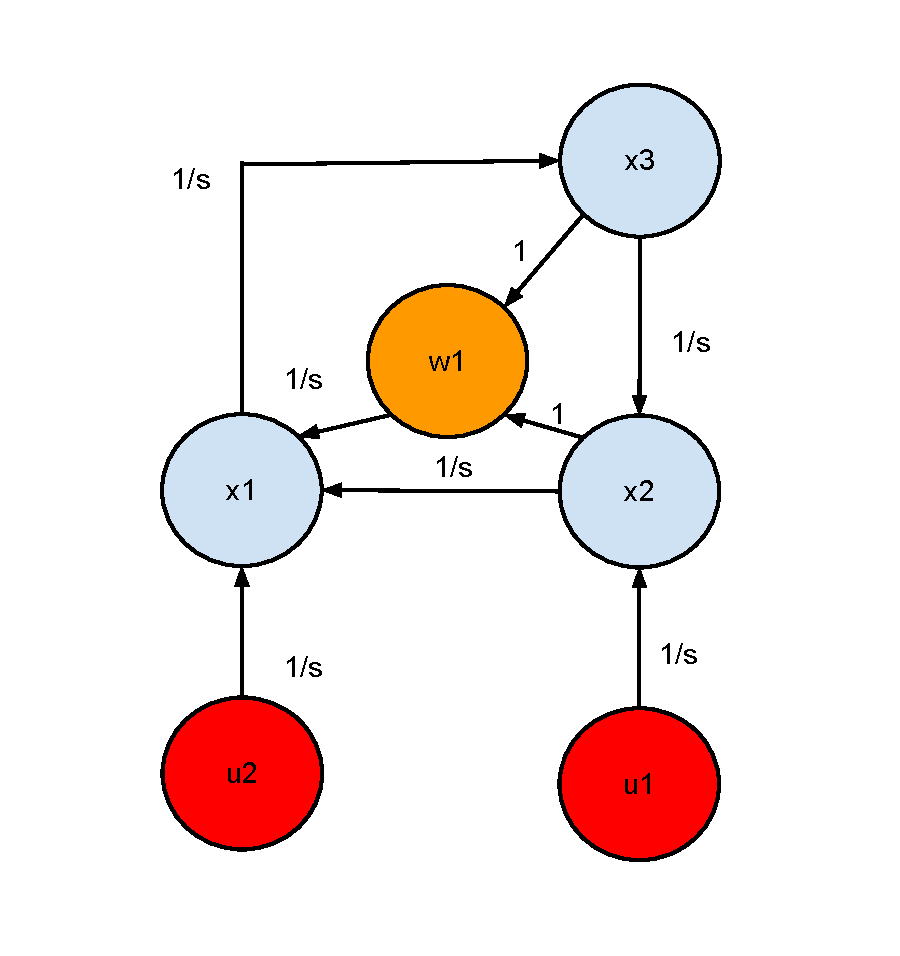
\includegraphics[scale=0.3,bb=0 0 153mm 162mm] {Figures/DAESFG.pdf}}\\\newline The ODE-representation of the same system would become:\\\newline
$\left[ \begin{array}{c} dx_1 \\ dx_2 \\ dx_3 \end{array} \right]
= \begin{bmatrix} 0 & 2 & 1 \\ 0 & 0 & 1 \\ 1 & 0 & 0 \end{bmatrix} \times \left[ \begin{array}{c} x_1 \\ x_2 \\ x_3 \end{array} \right] + \begin{bmatrix} 0 & 1 \\ 1 & 0 \\ 0 & 0 \end{bmatrix} \times \left[ \begin{array}{c} u_1 \\ u_2 \end{array} \right]$
\newline
$\left[ \begin{array}{c} w_1  \end{array} \right]
=  \begin{bmatrix} 0 & 1 & 1\end{bmatrix} \times \left[ \begin{array}{c} x_1 \\ x_2 \\ x_3 \end{array} \right] + \begin{bmatrix} 0 & 0 \end{bmatrix} \times \left[ \begin{array}{c} u_1 \\ u_2 \end{array} \right]$\newline Which then has the corresponding SFG:\newline
\setlength\fboxsep{0pt}
\setlength\fboxrule{0.5pt}
\fbox{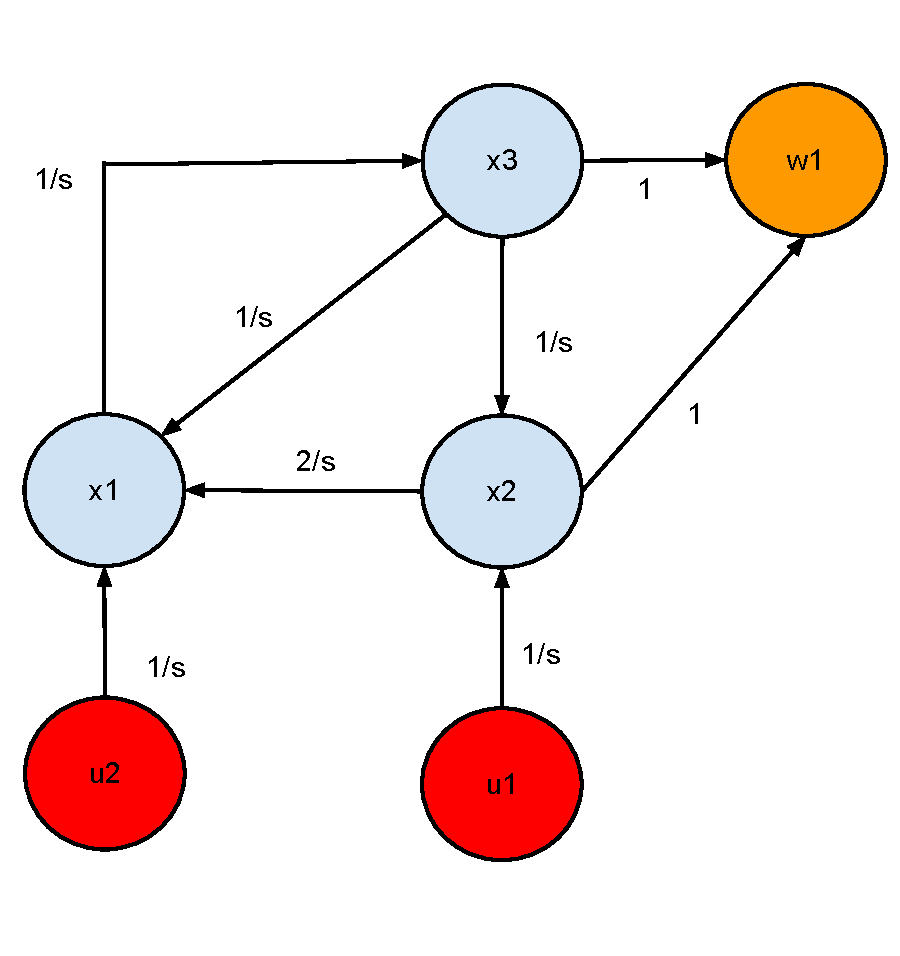
\includegraphics[scale=0.3,bb=0 0 153mm 162mm] {Figures/ODESFG.pdf}}\\\newline
As we can see, the SFG-representations of the two systems will differ, we no longer can see the relation between $x_1$ and $w_1$. This is a problem since a user might want to analyze the relation between the algebraic variable and other points in the system directly.
FIXME SHOULD THERE BE AN EXAMPLE OF SUCH A PROBLEM
%One such case would be the interconnection of three pipes.\\\newline
%
%\setlength\fboxsep{0pt}
%\setlength\fboxrule{0.5pt}
%\fbox{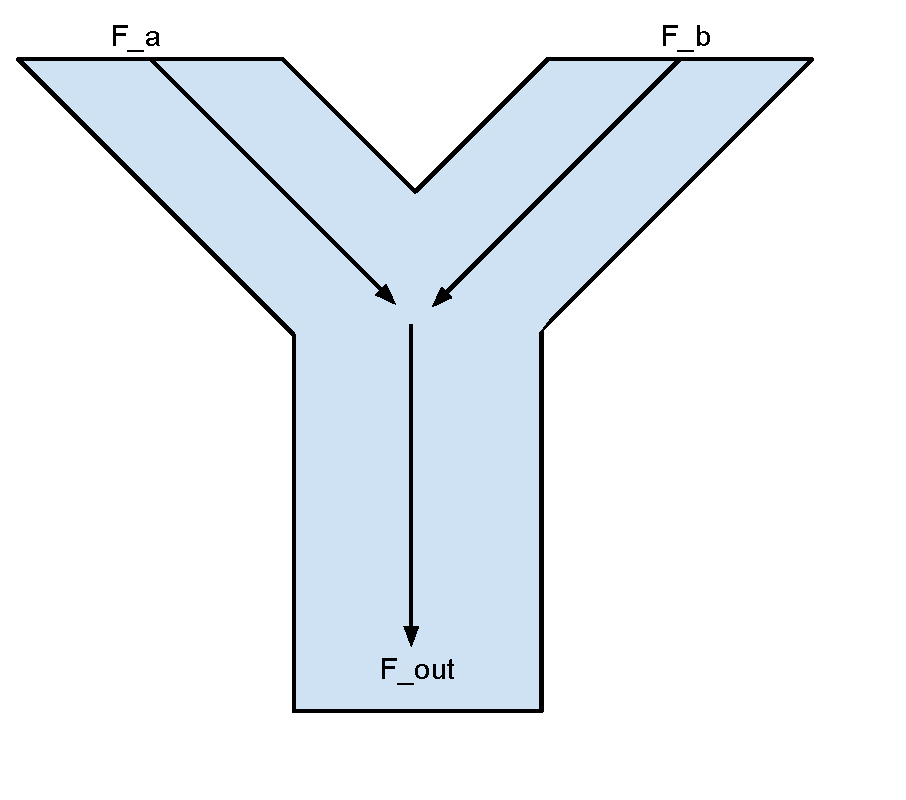
\includegraphics[scale=0.7,bb=0 0 154mm 136mm] {Figures/Apipe.pdf}}
%
%In a rough model, F_out is just the sum of the two flows, F_a and F_b. Still, the relation  
%
